\documentclass{article}

\usepackage{amsmath, amsfonts}
%\usepackage{tensor}
\usepackage[colorlinks]{hyperref}

\usepackage[format=plain,
            labelfont={bf,it},
            textfont=it]{caption}

\usepackage{graphicx, subcaption}
\graphicspath{ {./images/} }

% In terminal, run: biber strapdown_report
\usepackage[backend=biber]{biblatex}
\addbibresource{./strapdown_report.bib} %Import the bibliography file

\title{Strapdown integration for MEMS inertial sensors}
\author{Henk Luinge  \\
	infertia.com   \\
	}
	
\date{\today}

\begin{document}

\maketitle

\begin{abstract}
Applications using MEMS inertial sensors tend to use the movement signals at a much lower rate than the dynamics the movement, especially for movements that include impact or vibrations. This report describes a method for strapdown integration that preserves the integrated change in orientation and velocity the method by calculating it at a high rate and making it available to the user at a much lower rate. Rather than communicating gyroscope and accelerometer signals to the user application using a per-channel aliasing filter, it transmits a change in orientation and a change in acceleration. These incremental pose updates are computed on the IMU at a high internal frequency before being transmitted to the host. Reference code is provided.
\end{abstract}

\section{Introduction}


We consider applications in which a 3D inertial measurement unit (IMU) is used to track its change in movement. Were not only interested in the momentary sensor signals (angular velocity and accelerometer signals), but also in the integrated quantities: change in orientation, change in velocity and change in position. Typically these quantities are computed on a micro controller using a finite difference integration process also known as strap down integration, see e.g. Woodman \cite{Woodman2007}.

Small errors in sensor data as well as sampling artefacts will cause integration errors, leading to an increasing uncertainty in computed quantities. One specific error cause is loss of integrated values due to a too low strap down computation rate. In 3D movement, the change in orientation and velocity does not follow a simple linear integration, but a differential equation \cite{Bortz1970}. This means that a simple low-pass averaging filter is not sufficient to reconstruct the movement. 

In several applications in which movement is recorded using an IMU, the rate in which the user gets the data (ODR - output data rate) is lower than the dynamics as well as the internal sampling rate. 

Two examples:
\begin{itemize}
\item A wireless, foot-mounted IMU will record signals with a bandwidth of several hundreds of Hz. When using zigbee or bluetooth, the update rate will often be lower than 100Hz due to constraints in wireless transmission.
\item A MEMS IMU mounted on a vibrating mechanical construction can be subjected to vibrations in the kHz range. Because vibratory rotations can be coupled with translations, the strap down integration has to be solved at a rate higher than the Nyquist frequency. If the data is used as part of a controller, the controlled will generally operate on a lower sampling rate. 
\end{itemize}

In the above examples, if the strap down integration is done on the output data rate (ODR), the non commutativity problems can be a substantial part of the integration error, in particular when there is impact or vibrations.

With the amazing stability and linearity of modern IMU's (Bosch, TDK, ST MEMS gyroscopes and accelerometers), dealing with the strap down integration matters to reduce the integration drift and get more reliable movement sensing.

\begin{figure}[ht]
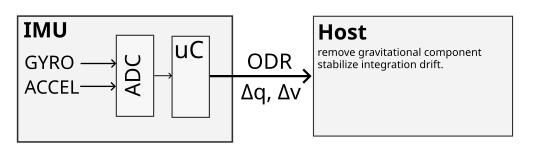
\includegraphics[scale=.8]{imu_and_host_diagram.png} 
\caption{Inertial sensors are sampled at a sufficiently high rate at the IMU side and the change in acceleration and velocity is computed. The IMU rate could be 1kHz depending on movement. The computed increments are then used by a host or user at a much lower ODR data rate. The host would take care of removing gravitational acceleration to compute the velocity and removing longer term integration drift.}
\centering
\label{fig:imu_host_diagram}
\end{figure}


A solution to the above problems is to compute the strap down integration over a short interval and send the change in orientation and change in velocity to a host, see figure \ref{fig:imu_host_diagram}. For the foot-mounted application with 10 Hz ODR, this could mean that an internal sampling rate of 1 kHz could be used. Then every 100 samples will be combined to a change in velocity and change in acceleration using strap down integration. These results will then be sent to the host with 10 Hz. Although the user will still have the signals at 10 Hz, there is no loss due to a low-rate strap down integration.

The document describes the implementation of the strap down integration that is divided up in a fast update section and a reduced rate section. The effect of sensing errors on the integration is not treated, nor a derivation of 3D kinematics to a finite difference equation. For reconstructing the velocity we assume a local tangent plane with fixed, known gravitational acceleration.

This report accompanies a jupyter notebook with the implementation. Emphasis is placed on creating an intuition between the equations describing the kinematics and the implementation. The content of the report is not new, it is intended to serve as a guide for implementation. This way of providing change in orientation/velocity rather than angular velocity/acceleration is already used by e.g. iMAR GmbH or Movella.

First, the general, well known strap down integration is introduced, as is proven for inertial sensors on a fixed local tangent plane. Then  the  equation is chopped up in a part that can be computed on the IMU part and a part that can run on the host.

\section{IMU sampling}
We assume a calibrated inertial measurement unit (IMU) that samples angular velocity and acceleration, each expressed as a vector along an coordinate system (S) attached to the IMU.

The signals are sampled at times $t_i$ with $i=1..ns$, $ns$ represents the number of samples used in the analysis.

Conventions:
\begin{itemize}
\item Time is measured at times $t_i$. The subscripts $t_i$, $t$ and $i$ are used interchangeably.
\item The first index (zero) is for the starting position, also in the python reference code. The starting position is assumed to be known. In practise, the first accel/gyro samples (index 0) are used to create an initial orientation estimate and it's uncertainty. Then the second sample (index 1) gives the first integration interval.
\end{itemize}


\section{Strap down integration for ideal sensors}

Define an ideal gyroscope and accelerometer, not corrupted by noise or calibration errors:
\begin{equation} \label{eq:ideal_gyroscope}
\begin{aligned}
\textbf{y}_{gyr, t} &= ^S \boldsymbol{\omega}_t  \\
\textbf{y}_{acc, t} &= ^S\boldsymbol{a}_t - ^S\boldsymbol{g}_t
\end{aligned} 
\end{equation}
with $\omega$ the angular velocity, $a$ the acceleration of the IMU and $g$ the gravitational component of acceleration.

We assume that the angular velocity $\boldsymbol{\omega}_t $ is constant during the sampling interval $t-T$ to and including t. Then the orientation change between two sampling times $t_{i-1}$ and $t_i$ is:

\begin{equation} \label{eq:single_sample_angular_velocity_integration}
\boldsymbol{\delta q}_i = \begin{bmatrix}
cos(\left| \omega_i \right|/2) \\ 
sin(\boldsymbol{\omega_i}/2)
\end{bmatrix} = exp(\boldsymbol{\omega_i}/2) =exp(\boldsymbol{y}_{gyr,i}/2)
\end{equation}

The subscript $i$ is used to indicate the time $t_i$ and the left superscript specifies the coordinate frame the vector is expressed.
The orientation change up to sample $j$ at time $t_j$ is obtained by concatenating the orientation differences:

\begin{equation} \label{eq:angular_velocity_integration}
^{LS}\textbf{q}_{j}={}^{LS}\boldsymbol{q}_0 \cdot \prod_{i=1}^{j}\boldsymbol{\delta q}_i
\end{equation}

or in recursive form, omitting the starting orientation: 
\begin{equation} \label{eq:angular_velocity_integration_recursive}
^{LS}\textbf{q}_i= ^{LS}\textbf{q}_{i-1} \cdot \boldsymbol{\delta q}_i
\end{equation}

The multiplication dot between two quaternions is the quaternion multiplication, implemented in the python/kinematics algebra module, see also e.g. \href{http://lisyarus.github.io/blog/posts/introduction-to-quaternions.html}{lisyarus}. Due to the non-commutativity, equation (\ref{eq:angular_velocity_integration}) must be evaluated in order of increasing time.

L represents a non-moving inertial coordinate system. It can be the local tangent plane,  or lab coordinate system, or it can be the coordinate system of the device at start of recording.

To compute the velocity, the acceleration is integrated, assuming the acceleration was constant over the period $t_{i-1}..t_i$.

\begin{equation} \label{eq:acceleration_integration}
\begin{aligned}
^L\textbf{v}_i &= ^L\textbf{v}_{i-1} + T \cdot ^L\boldsymbol{a}_i \\
&=  ^L\textbf{v}_{i-1} + T \cdot ^L\boldsymbol{y}_{acc,i} + T \cdot ^L \boldsymbol{g} \\
&=  ^L\textbf{v}_{i-1} + T \cdot{}^{LS}\boldsymbol{R}_i \cdot ^S\boldsymbol{y}_{acc,i} + T \cdot ^L \boldsymbol{g}
\end{aligned} 
\end{equation}

or in direct form:

\begin{equation} \label{eq:acceleration_integration_sum}
^L\textbf{v}_{j}= ^L\textbf{v}_0 + T \sum_{i=1}^{j} {}^{LS}\boldsymbol{R} \cdot \boldsymbol{y}_{acc,i} +ns \cdot T \cdot ^L\boldsymbol{g}
\end{equation}

In case the local L frame is defined with Z-axis upwards  the gravity is described as:
\begin{equation} \label{eq:gravity_down}
^L\textbf{g} = \begin{bmatrix} 0 & 0 & -g_c \end{bmatrix}^T
\end{equation}
with $g_c$ the local gravitational constant, e.g. $9.81 m/s^2$ in the Netherlands.

\section{Sectioning the integral}

Define the following \textbf{time instants}:
\begin{itemize}
\item High-frequency sampling times $t_i$ with  $i \in 0..n_t$. This would typically be the rate of the ADC converter, at a rate of hundreds to perhaps thousands of Hz. L would represent the current time that the pose needs to be calculated.
\item the time instants of the output data rate. These are given by $D_j$ with  $j \in 0..n_j$. j starts at zero and grows with the duration of the measurement. M would be the pose at current time: $t_{nt}=D_{nj}$
\item High frequency sampling times within the interval $s_k$ with  $k \in 0..n_k$. The index $k$ resets with every new ODR interval.
\end{itemize}

Define the following \textbf{intervals}:
\begin{itemize}
\item The change in velocity or change in orientation over a short interval from $s_{k-1}$ to $s_k$ is given by $\delta_k$.
\item The change in velocity or change in orientation over an ODR interval from $D_{j-1}$ to $D_j$ is given by $\Delta_j$.
\end{itemize}

We assume that when an signal such as accelerometer signal $y_{acc}$ is measured at some time $t_i$, it was constant between $t_{i-1}$ and $t_i$.

A graphical summary of the above is vien in figure \ref{fig:strapdown_integration_timelines}.

\begin{figure}[ht]
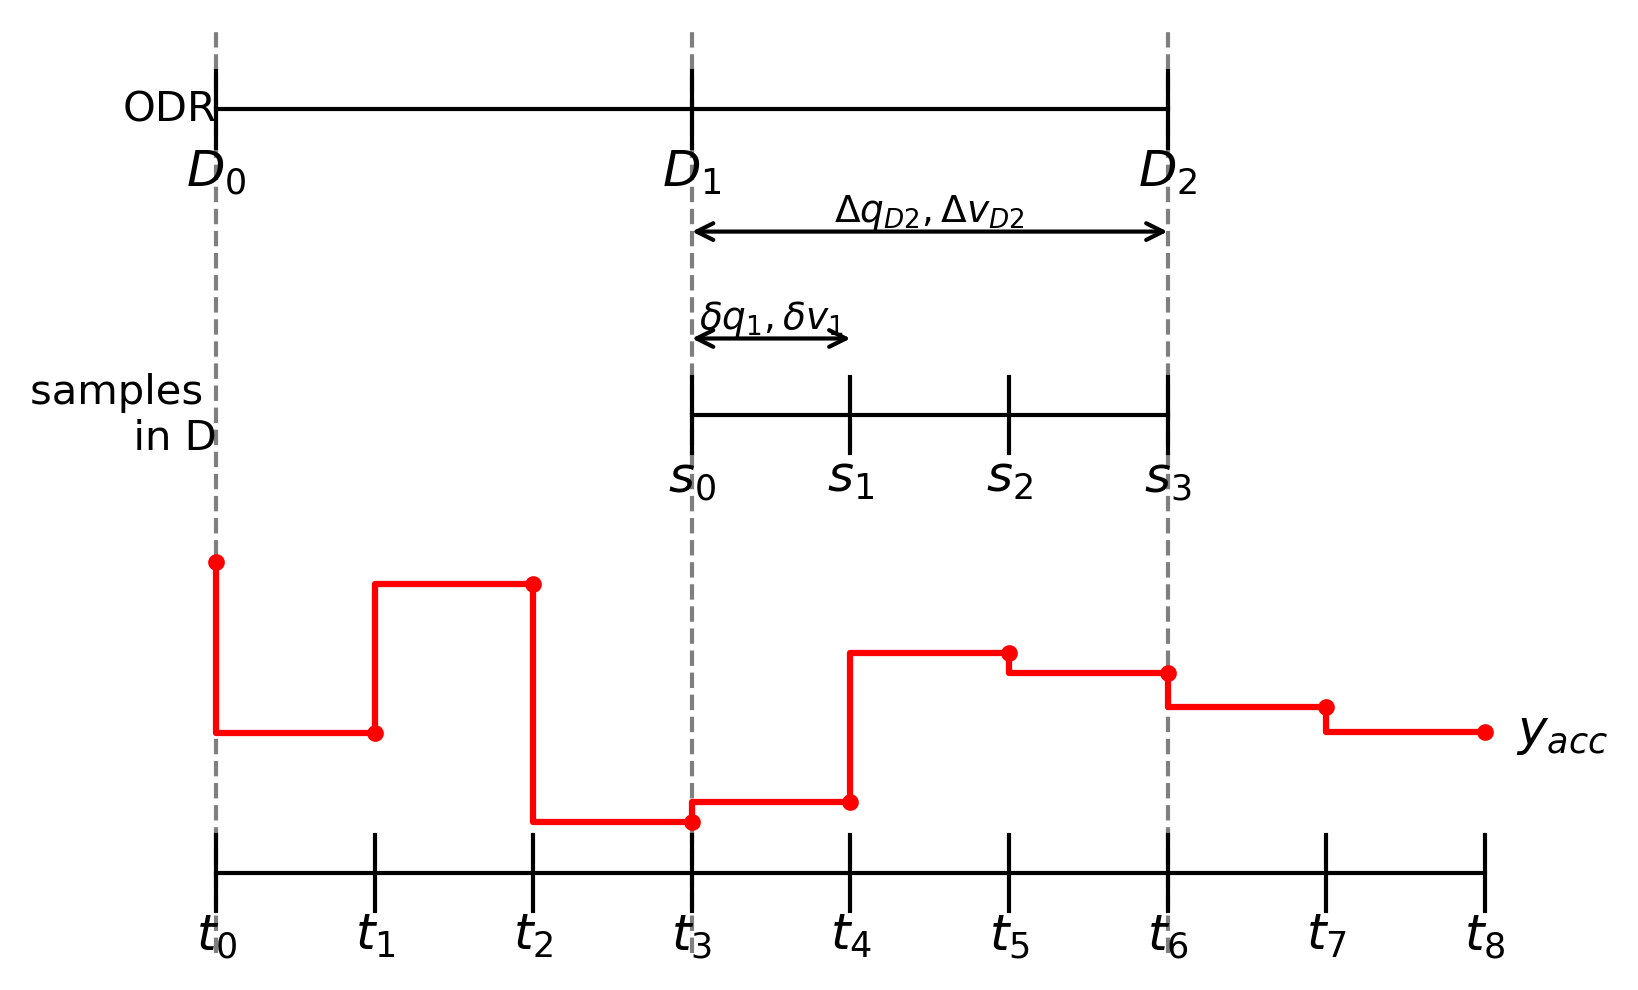
\includegraphics[scale=.8]{strapdown_integration_timelines.png} 
\caption{Definition of timelines and intervals.  We seek to capture integrated quantities from each ODR interval ($D_0$, $D_1$,...). The samples within the ODR interval are written as $s_i$.}
\centering
\label{fig:strapdown_integration_timelines}
\end{figure}

Following from \ref{eq:angular_velocity_integration}, the orientation at some time $t=t_L$ is chopped up in two multiplication sequences:
\begin{equation} \label{eq:orientation_chopped_up}
^{LS_t}\textbf{q}_{} = \prod_{j=1}^{n_j}\boldsymbol{\Delta q}_j
= \prod_{j=1}^{n_j} \prod_{k=1}^{n_k} \boldsymbol{\delta q}_k
\end{equation}

Similarly following \ref{eq:angular_velocity_integration}, the change in velocity at the end of ODR interval j:
\begin{equation} \label{eq:acceleration_chopped_up}
\begin{aligned}
^L\textbf{v}_{j} &= ^L\textbf{v}_0 + T \sum_{j=1}^{n_j} \sum_{k=1}^{n_k} {}^{LS}\boldsymbol{R} \cdot \boldsymbol{y}_{acc,i} +n_{j} \cdot n_s \cdot T \cdot ^L\boldsymbol{g} \\ 
&=  ^L\textbf{v}_0 + T \sum_{j=1}^{n_j} \Delta v_t + n_{j} \cdot n_s \cdot T \cdot ^L\boldsymbol{g}
\end{aligned}
\end{equation}

In recursive format, again omitting the starting velocity:
\begin{equation}
^L\textbf{v}_t = ^L\textbf{v}_{t-1} + \Delta \textbf{v}_t +  n_s \cdot T \cdot ^L\boldsymbol{g}
\end{equation}

\subsection{On-imu calculations}
Using the quantities that can be computed on the IMU, the change in orientation in and interval j, using samples i=1..ns within that interval:

\begin{equation} \label{eq:deltas}
\begin{aligned}
\Delta \boldsymbol{q}_j &= \prod_{i=1}^{ns} exp(T\boldsymbol{y}_{gyr,i}/2)\\
\Delta v_j &=  T \sum_{i=1}^{n_s} {}^{LS}\boldsymbol{R}_i \cdot \boldsymbol{y}_{acc,i} 
\end{aligned}
\end{equation}

\section{Benefit}

\subsection{Coning motion}
The performance increase depends on the movement: more 1 dimensional rotations give less noncommutativiy errors than movements in which the direction of rotation is changing. As a test case we use coning motion, sometimes called helical motion. The orientation change is defined by 

\begin{equation} \label{eq:coning_angular_velocity}
\boldsymbol{\omega}(t) = \omega \begin{bmatrix}
\sin \theta \cdot cos(\omega t) \\
-\sin \theta \cdot \sin(\omega t) \\
 (1 - cos \theta)
\end{bmatrix}
\end{equation}

The coning motion is interesting because the angular velocity is constantly changing direction and therefore challenging. For the illustration, we use $\theta=\pi /2$ to maximimize the coning effect and  $\omega=2[Hz] \cdot 2\pi$, corresponding to e.g. a brisk walk.

\begin{figure}[ht]
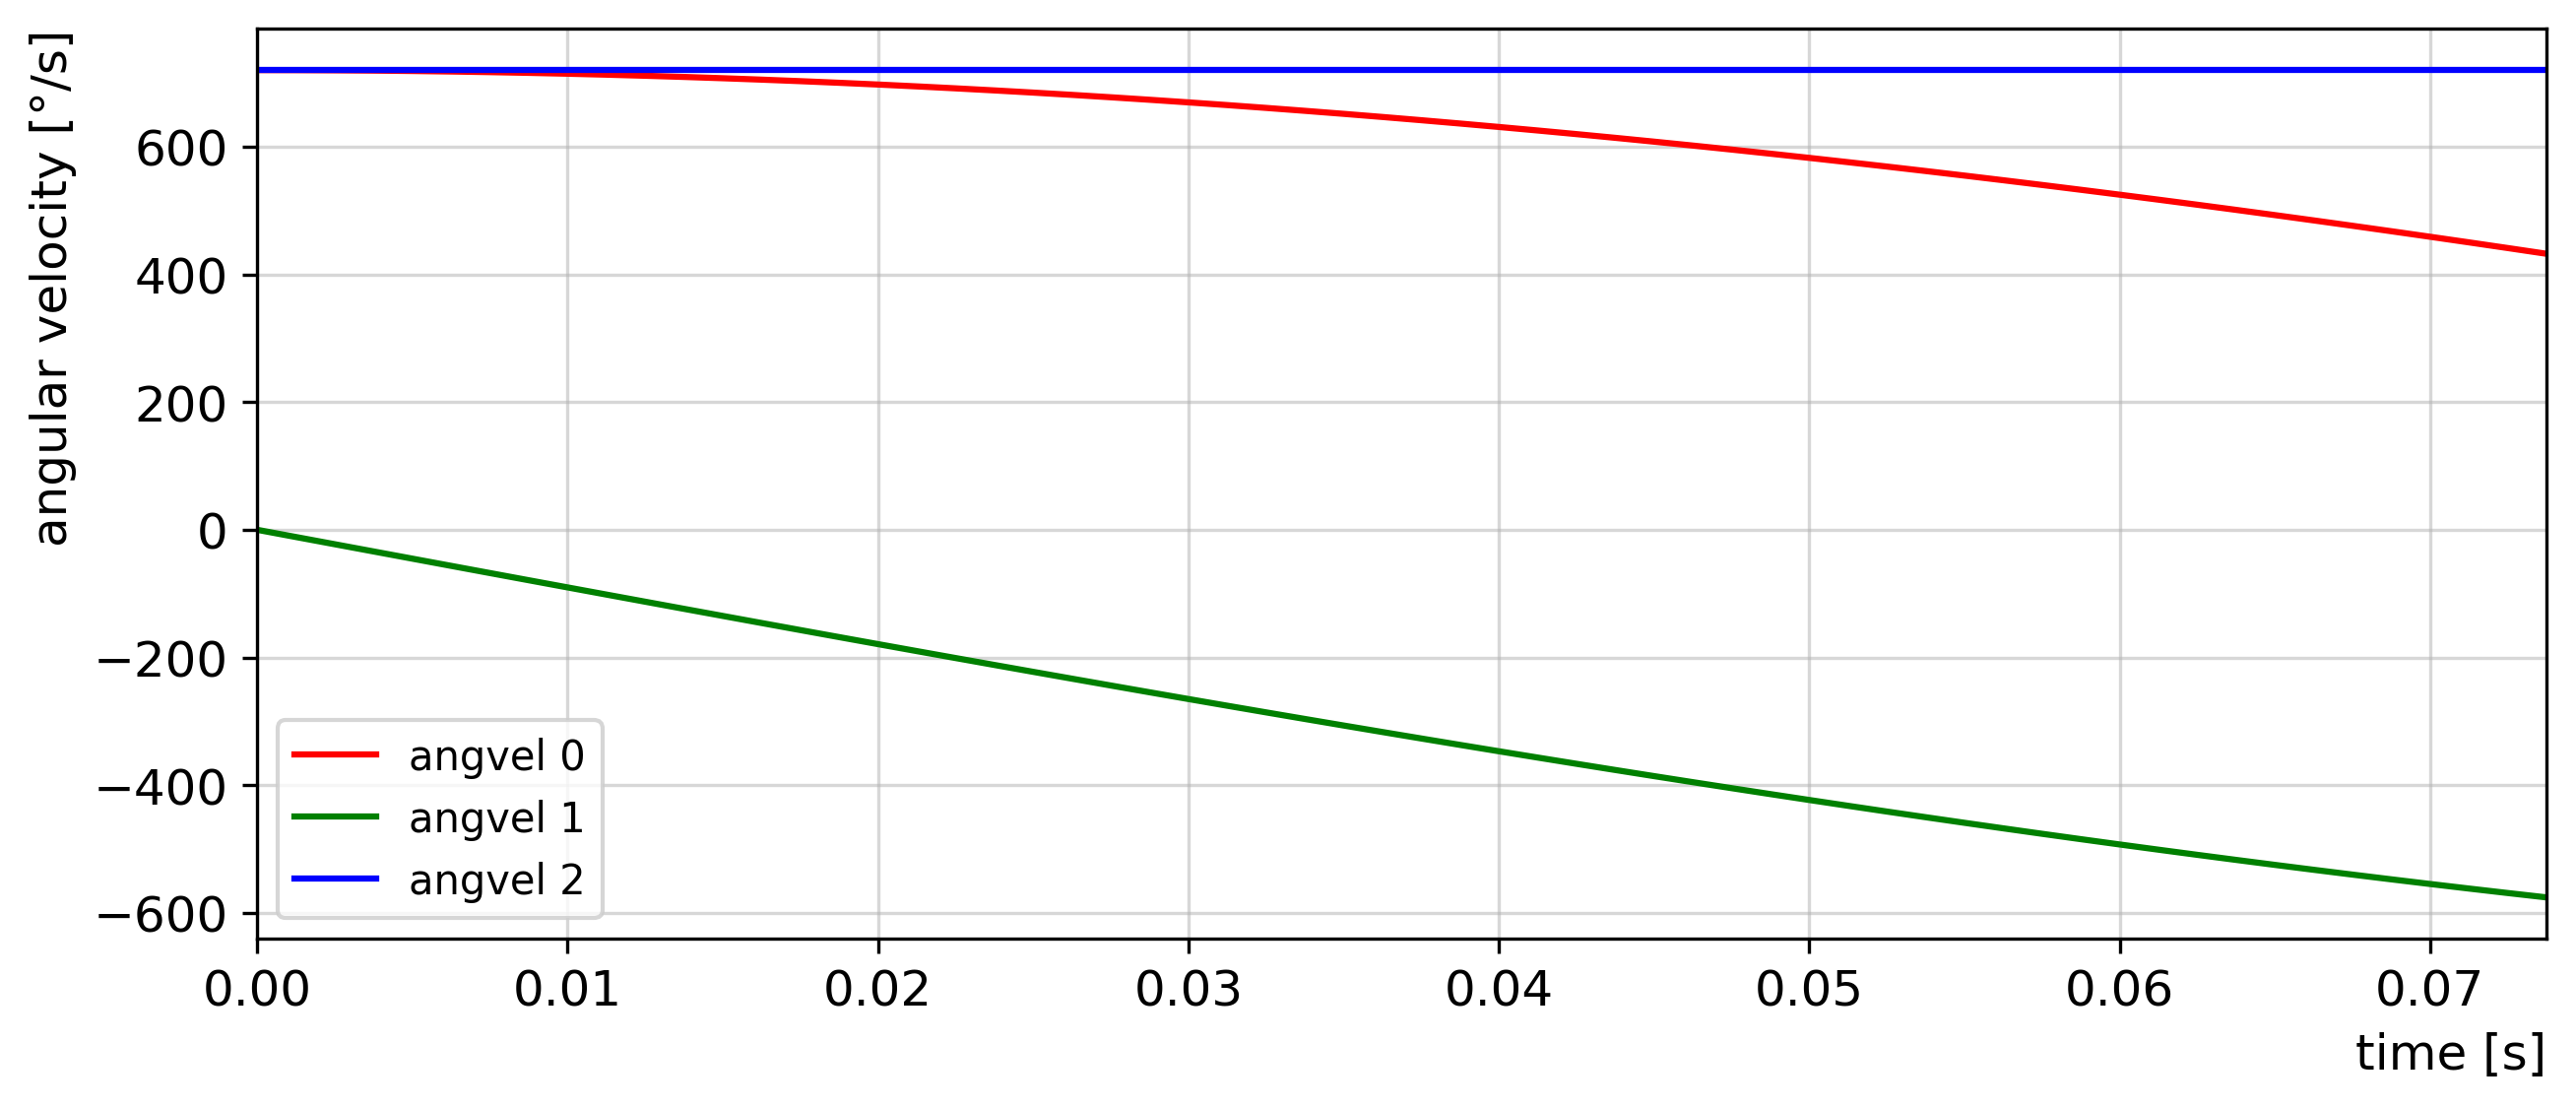
\includegraphics[width=.9\textwidth]{angular_velocity_coning.png} 
\caption{Coning angular velocity with duration 4[s], $theta=\pi /2$, $\omega=2\cdot 2 \pi$, corresponding to 2Hz.}
\centering
\end{figure}


\subsection{Effect of ODR}
The effect of on-IMU strapdown integration is illustrated in figure \ref{fig:effect_of_odr}. Two strapdown integration mechanizations are compared:
\begin{itemize}
\item on-IMU strap down integration of 800 Hz, then output to the host on the frequency specified by ODR (dashed line). The host then concatenates the change in velocity and change in acceleration as described above.
\item A mechanization in which the average gyroscope/accelerometer signal during an ODR sampling period is transmitted to the host. The host then properly integrates the angular velocity and acceleration assuming a constant angular velocity/acceleration during the sampling interval. This case is representative of an anti aliasing filter on each of the sensor signals.
\end{itemize}

Particularly for update rates below 40Hz, the coning effect can become too large to be useful. With on-IMU strapdown integration, the strap down integration errors are determined by the internal sampling frequency which can  in general be chosen sufficiently high - in this case 800Hz.

\begin{figure}[ht]
\centering
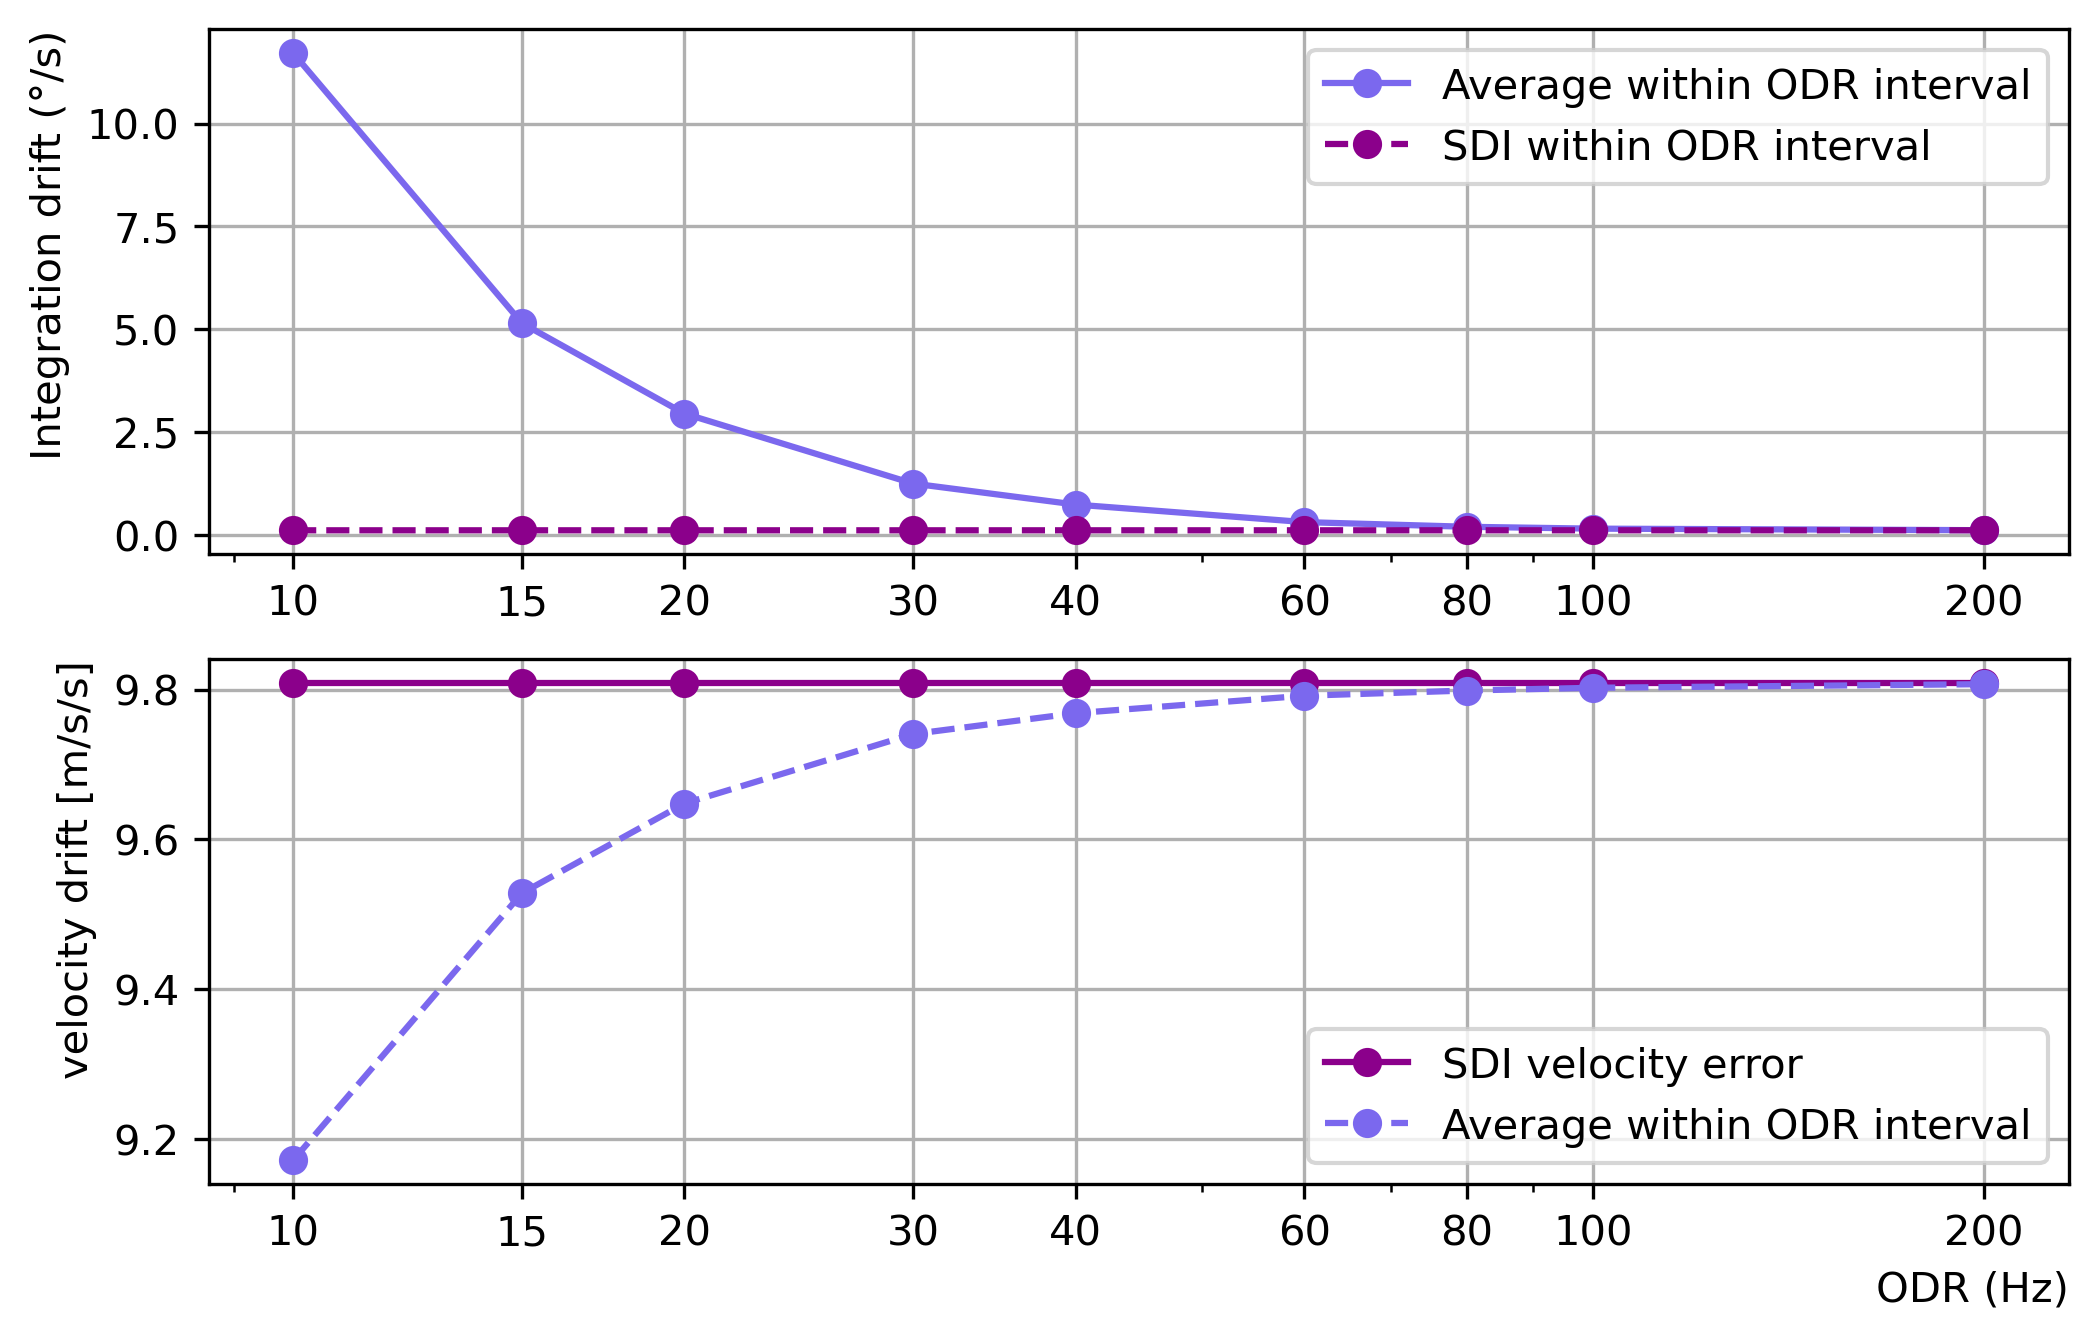
\includegraphics[width=0.9\textwidth]{drift_versus_odr_frequency.png} 
\caption{Effect of on-IMU strap down integration is largest for low communication rates.}
\label{fig:effect_of_odr}
\end{figure}

A 20Hz update rate could be sufficient for visualization purposes or perhaps a motor control application. Still due to sampling alone, the integration drift can be significant. If then inevitable sensors errors such as calibration errors and noise are present, the drift will quickly be a limitation to accurate pose tracking.


\printbibliography

\end{document}
